

\section{Анализ работы фонтанирующей скважины}

При достаточном количестве естественной энергии скважина может фонтанировать. Инженерные расчеты требуются как для оптимизации работы самого подъемника, так и системы "скважина-пласт".

Для упражнения требуется задать PVT свойства флюидов, конструкцию скважины, свойства пласта и текущий режим работы скважины (дебит). Все исходные данные заполняются аналогично предыдущим упражнениям за исключением функции, объединяющей все данные о скважине в одну строку, расположенной в ячейке  $G23$

{ \small  \texttt{=well\_encode\_string(Hmes\_;Htube\_;Udl\_;Dcas\_;Dtub\_;0;;Twf\_;Tbuf\_)
}}

\begin{figure}[h!]
	\center{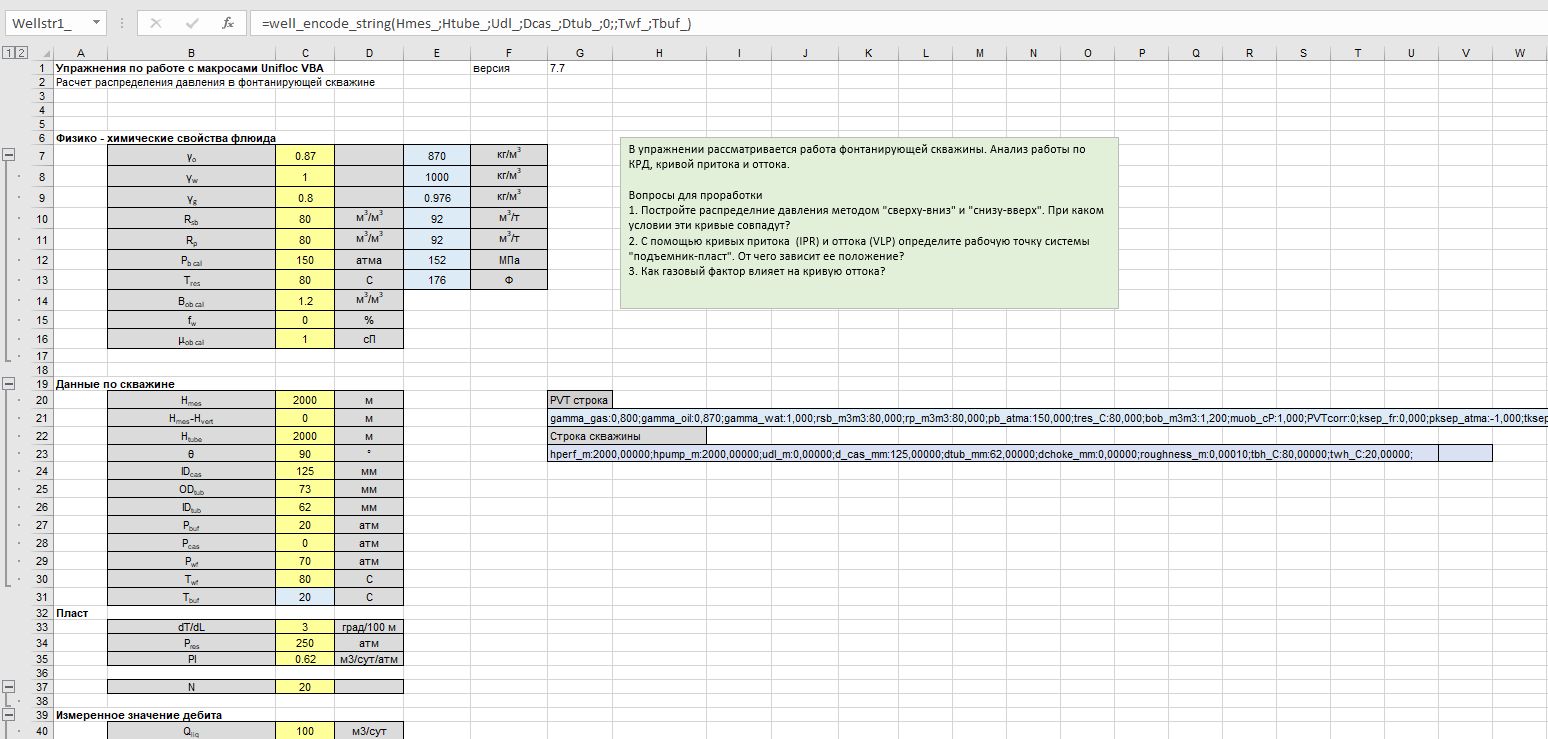
\includegraphics[width=1\linewidth]{Ex90_1}}
	\caption{Исходные данные для расчета фонтанирующей скважины}
	\label{ris:Ex90_1}
\end{figure}

В первой части задания требуется построить распределение давления в скважине методом сверху-вниз и снизу-вверх, задавая при этом граничные условия - давление на устье и на забое соответственно. Для расчета воспользуйтесь в ячейке $E50$ функцией

{ \small  \texttt{=MF\_p\_pipe\_atma(Qtest\_; fw\_;C49; C50;E49;PVRstr1\_; theta\_;Dtub\_;;D49;D50)
}}

"протянув"\ ее на весь столбец. Расчет снизу-вверх выполните аналогичным образом. Обратите внимание, что при правильных расчетах КРД должны совпадать - решение не должно зависеть от направления.

\begin{figure}[h!]
	\center{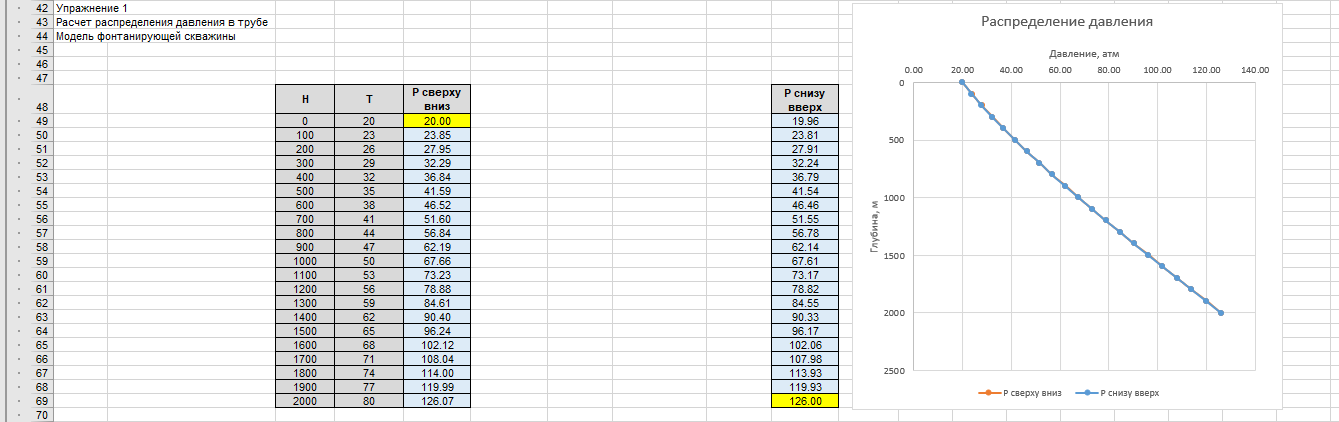
\includegraphics[width=1\linewidth]{Ex90_2}}
	\caption{Расчет КРД в фонтанирующей скважине}
	\label{ris:Ex90_2}
\end{figure}

Во второй части упражнения необходимо построить кривую притока (индикаторную кривую, по Вогелю) и кривую оттока (зависимость давления в начале подъемной трубы от дебита при неизменном давление на выходе). Забойное давление принимается равным рассчитанному из предыдущей части упражнения. Максимальный дебит скважины и коэффициент продуктивности можно варьировать вместе с обводненностью продукции скважины для анализа добывающей системы. Точка пересечения кривых притока и оттока будет являться рабочей точкой системы "пласт-скважина".

Для вычисления забойного давления для индикаторной кривой воспользуйтесь в ячейке $F78$ уже знакомой Вам функцией

{ \small  \texttt{=IPR\_Pwf\_atma(PI\_1;Pres\_;E78;fw\_;Pb\_)}}

Расчет забойного давления по устьевому в ячейке $G78$ примените функцию
 
{ \small  \texttt{=well\_pwf\_plin\_atma(E78;fw\_;Pbuf\_; Pcas\_; Wellstr1\_; PVRstr1\_; ;1;;;;;;1)}} 

Для другой величины обводненности продукции в $H78$ при анализе дальнейшей работы

{ \small  \texttt{=well\_pwf\_plin\_atma(E78;fw\_2;Pbuf\_; Pcas\_; Wellstr1\_; PVRstr1\_; ;1;;;;;;1)}} 

Заполнив таблицу до конца Вы получите следующий результат

\begin{figure}[h!]
	\center{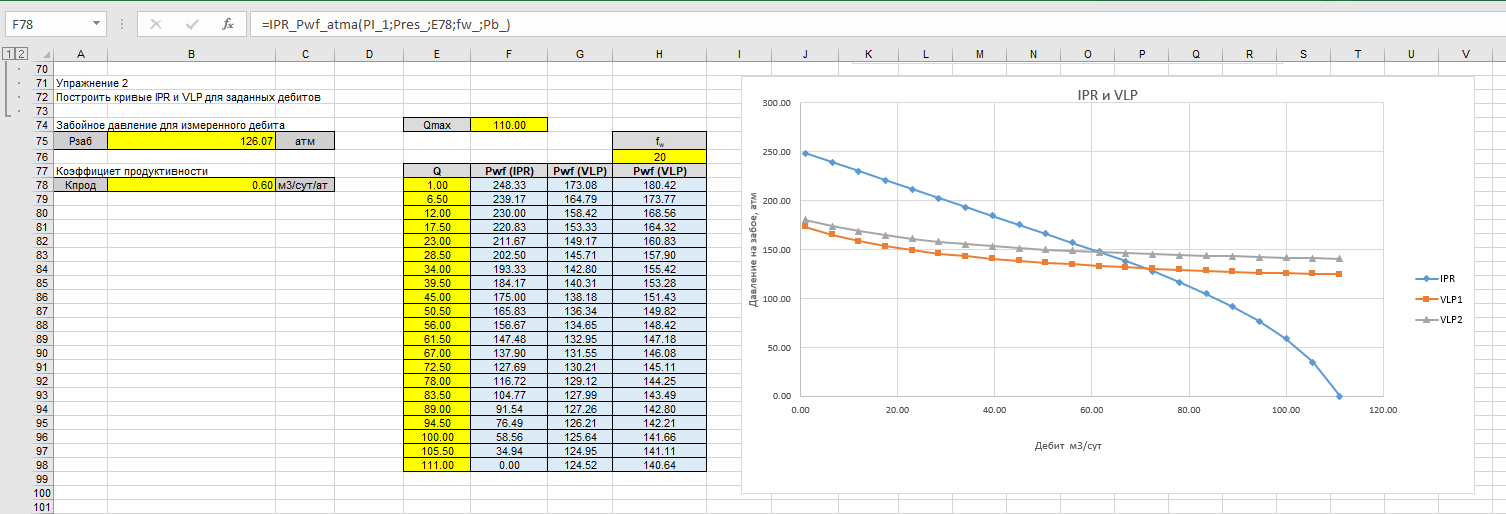
\includegraphics[width=1\linewidth]{Ex90_3}}
	\caption{Кривые оттока и притока для узлового анализа работы фонтанирующей скважины}
	\label{ris:Ex90_3}
\end{figure}

Для анализа влияния ГФ скважины на забойное давление воспользуйтесь теми же самыми функциями, за исключением того, что каждый раз будет меняться PVT строка свойств флюидов

В ячейке $H108$ 

{ \small  \texttt{=well\_pwf\_plin\_atma(Qtest\_;fw\_;Pbuf\_;Pcas\_;Wellstr1\_;G108;;1;;;;;;1)}}

В ячейке $I108$ 

{ \small  \texttt{=well\_pwf\_plin\_atma(Qtest\_;fw\_3;Pbuf\_;Pcas\_;Wellstr1\_;G108;;1;;;;;;1)}}

\begin{figure}[h!]
	\center{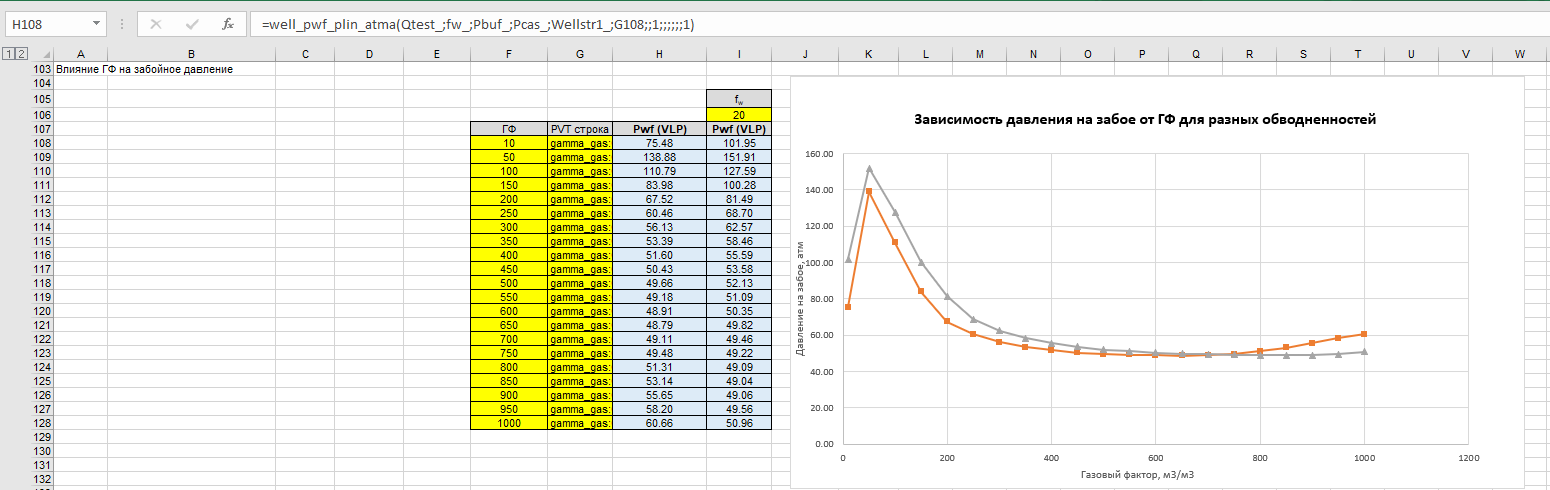
\includegraphics[width=1\linewidth]{Ex90_4}}
	\caption{Влияние газового фактора и обводненности на забойное давление}
	\label{ris:Ex90_4}
\end{figure}

Теперь Вы можете ответить на вопросы:

Вопросы для проработки

\begin{enumerate}
	\item Постройте распределние давления методом сверху-вниз и снизу-вверх. При каком условии эти кривые совпадут?
	\item С помощью кривых притока  (IPR) и оттока (VLP) определите рабочую точку системы "скважина-пласт". От чего зависит ее положение?
	\item Как газовый фактор влияет на кривую оттока?
\end{enumerate}

\section{Анализ работы скважины, оснащенной УЭЦН}

По сравнению с моделью фонтанирующей скважины в данный расчет добавляются такие важные элементы, как сепарация на приеме погружного оборудования и напорная характеристика ЭЦН. К стандартным исходным данным добавляется вторая PVT строка ($G45$) для разделения упражнения на 2 части. 

{ \small  \texttt{=PVT\_encode\_string(gamma\_gas\_; gamma\_oil\_; ; Rsb\_; Rp\_; Pb\_; Tres\_; Bob\_; mu\_;; KsepGasSep\_; PKsep2; TKsep2)
}}

Стоит сразу отметить важность определения давления и температуры, при которой происходит сепарация газа в затрубное пространство. При неизвестном давлении на приеме погружного оборудования (давлении сепарации) требуется определить его с помощью гидравлической корреляции, например, при расчете снизу-вверх от забойного давления. Однако расчет перепада давления в трубе зависит от PVT свойств, в том числе давления сепарации - поэтому требуется итеративный подход для изменения давления сепарации до тех пор, пока оно не окажется стабильным (и равным давлению на приеме погружного оборудования по гидравлической корреляции). Т.к. при сепарации происходит модификация флюида, пренебрежение согласованностью приведет к неправильному расчету - поток может быть дегазированным на забое или наоборот с высокой долей газа в насосе или НКТ. Изменять давление сепарации $P_{sep}$ можно в ячейке $C43$

\begin{figure}[h!]
	\center{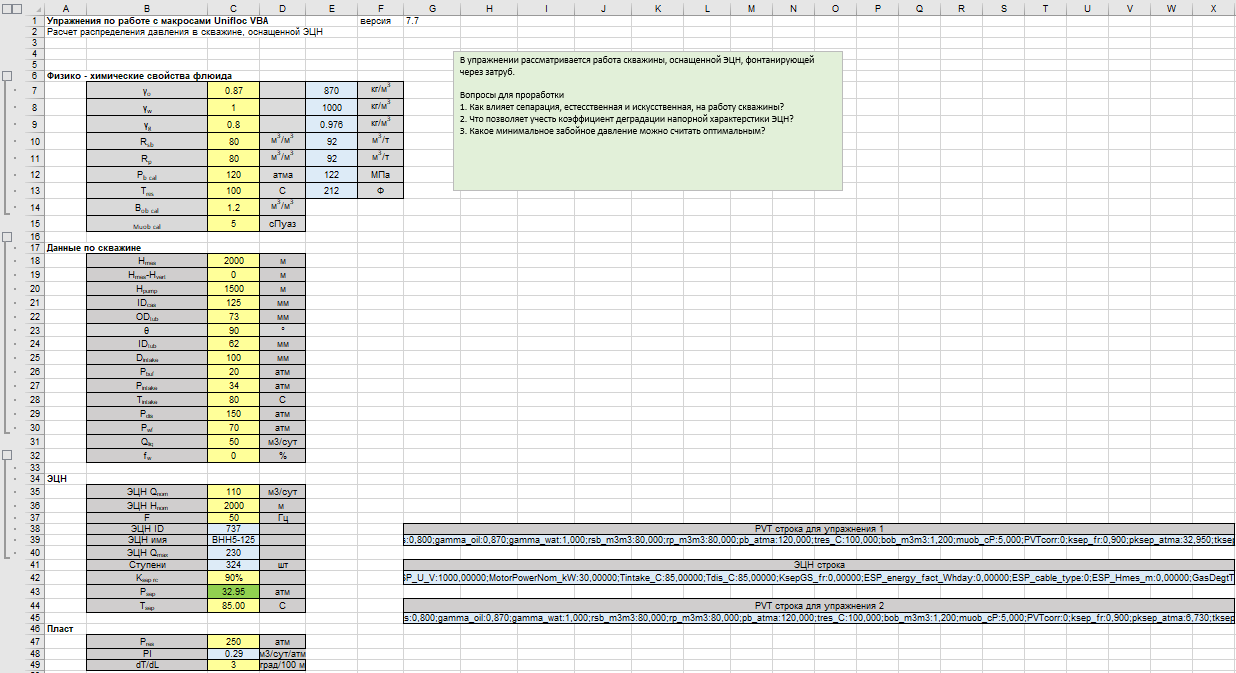
\includegraphics[width=1\linewidth]{Ex100_1}}
	\caption{Исходные данные для расчета скважины, оснащенной УЭЦН}
	\label{ris:Ex100_1}
\end{figure}

В первой части упражнения предлагается построить распределение давления в скважине с постоянным дебитом. 

Кривую давления от забоя до приема можно получить с помощью функции

{ \small  \texttt{=MF\_p\_pipe\_atma(Q\_;fw\_;C83;C82; F83;PVT\_str\_; theta\_; Dtub\_;; D83;D82)
}}

"протянув"\ ее до глубины спуска оборудования. С учетом сепарации, которая подробно описывалась выше, требуется изменять значение давления сепарации $P_{sep}$ в исходных данных ($C43$) пока оно не станет равным расчетному.

Затем в ячейке $G78$ можно определить коэффициент естественной сепарации

{ \small  \texttt{=MF\_ksep\_natural\_d(Q\_; wc\_; Pintake\_; Tintake\_; Dintake\_; Dcas\_; PVT\_str\_)
}}

А в $H78$ искусственную с помощью 

{ \small  \texttt{=MF\_ksep\_total\_d(G78;KsepGasSep\_)
}}

Распределение давления в НКТ рассчитывается методом сверху-вниз, начиная с ячейки $K64$

{ \small  \texttt{=MF\_p\_pipe\_atma(Q\_;fw\_;C63;C64;K63;PVT\_str\_;theta\_;Dintake\_;;D63;D64)
}}

Таким образом можно получить перепад давления в насосе не прибегая к расчету самого насоса - он будет равен разнице между давлением в нижней точке НКТ и на приеме погружного оборудования (ячейка $N78$). Но по напорной характеристике с помощью функции в $M78$

{ \small  \texttt{=ESP\_dP\_atm(Q\_; fw\_;Pintake\_; NumStage\_;Freq\_; PumpID\_; PVT\_str\_;Tintake\_; 0;1;;D60)
}}

также можно получить данное значение, воспользовавшись коэффициентом деградации напорной характеристики ЭЦН в $D60$ для адаптации модели. При совпадении результатов двух независимых расчетов возможно оценить состояние погружного оборудования.

Полезным для анализа работы добывающей системы будет знание о доли газа в потоке как до приема погружного оборудования (начиная с ячейки $I83$)

{ \small  \texttt{=MF\_gas\_fraction\_d(F83;D83;fw\_;PVT\_str\_)
}}

так и после сепарации в НКТ (с $J78$)

{ \small  \texttt{=MF\_gas\_fraction\_d(K78;D78;fw\_;PVT\_str\_)
}}

На этом первая часть упражнения завершается.

\begin{figure}[h!]
	\center{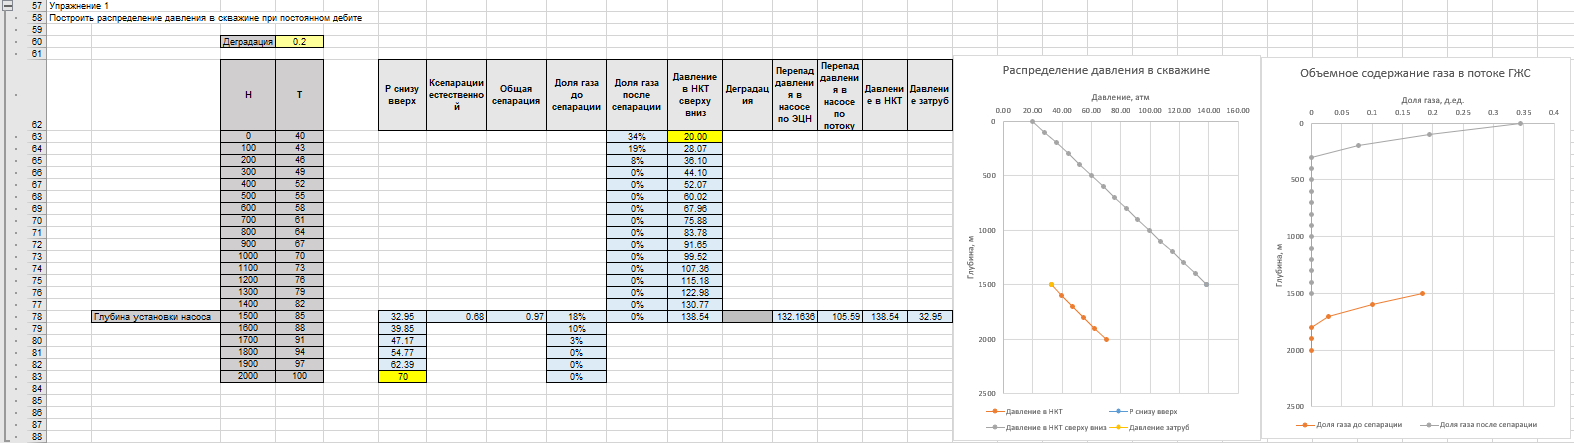
\includegraphics[width=1\linewidth]{Ex100_2}}
	\caption{Распределение давления в скважине с постоянным дебитом}
	\label{ris:Ex100_2}
\end{figure}

Во второй части упражнения распределение давления скважины строится с учетом того, что она имеет постоянную продуктивность. Изменение забойного давления в ячейке $D92$ приведет к изменению дебита скважины. Также могут варьироваться давление сепарации, коэффициент деградации и частота ЭЦН для настройки модели.

Сам расчет ведется только методом снизу-вверх: по забойному давлению определяется давление на приеме, затем вместе с коэффициентом сепарации рассчитывается перепад давления в насосе по напорной характеристике, а после устьевое давление по давлению на выходе насоса, начиная с ячейки $K114$ c помощью функции

{ \small  \texttt{=MF\_p\_pipe\_atma(Qreal\_; fw\_;C115;C114; K115;PVT\_str\_2;theta\_; Dintake\_;; D115; D114)
}}

При этом PVT строка будет использоваться другая из-за отличных значений давления на приеме по сравнению с первой частью упражнения.

\begin{figure}[h!]
	\center{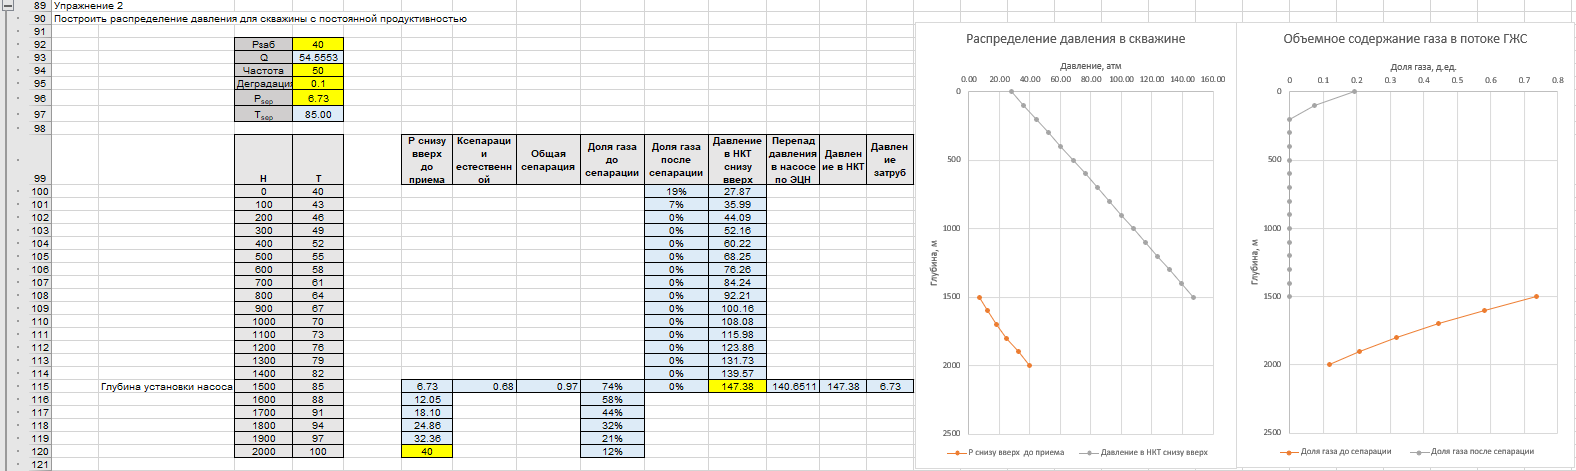
\includegraphics[width=1\linewidth]{Ex100_3}}
	\caption{Распределение давления в скважине с постоянной продуктивностью}
	\label{ris:Ex100_3}
\end{figure}

С помощью дополнительных исследований (при необходимости) ответьте на вопросы

\begin{enumerate}
	\item Как влияет сепарация, естественная и искусственная, на работу скважины?
	\item Что позволяет учесть коэффициент деградации напорной характеристики ЭЦН?
	\item Какое минимальное забойное давление можно считать оптимальным?
\end{enumerate}


\section{Анализ работы скважины, оснащенной ЭЦН, фонтанирующей через затрубное пространство}

Общая теория 

При спуске погружного оборудования в фонтанирующую скважину с большим газовым фактором газожидкостный поток у приема может разделяться на 2 составляющие: поток с низким газосодержанием после сепарации естественной и искусственной в НКТ и поток с большой долей свободного газа в затрубное пространство. 

При этом ЭЦН за счет энергии движения ГЖС работает практически на холостом ходу, развивая обычный перепад давления по напорной характеристике. Также при дебите большем, чем максимально возможный перепад давления  насоса, может происходить турбинное вращение, насос будет работать как гидравлическое сопротивление. Перегрев электродвигателя не происходит, т.к. он непрерывно охлаждается общим газожидкостным потоком.

В затрубном пространстве за счет большого количество газа будет происходить фонтанирование. Давление в затрубном пространстве будет большим, чем буферное, потому как обратный клапан в затрубе, предназначеныый для сброса газа, с жидкостью будет функционировать как штуцер, дросселируя давление. Без обратного клапана можно сделать  логичное предположение о том, что давления будут равными - газлифтный эффект в затрубном пространстве (подъем газожидкостной смеси за счет снижения плотности) будет равен перепаду давления, который создает ЭЦН.

Отсюда возникает вопрос, рационально ли устанавливать ЭЦН в фонтанирующую скважину с большим газовым фактором?

В данном упражнении предлагается смоделировать данный процесс. Но Вы также можете просмотреть расширенный расчет реальной скважины в папке "аpp".

\begin{figure}[h!]
	\center{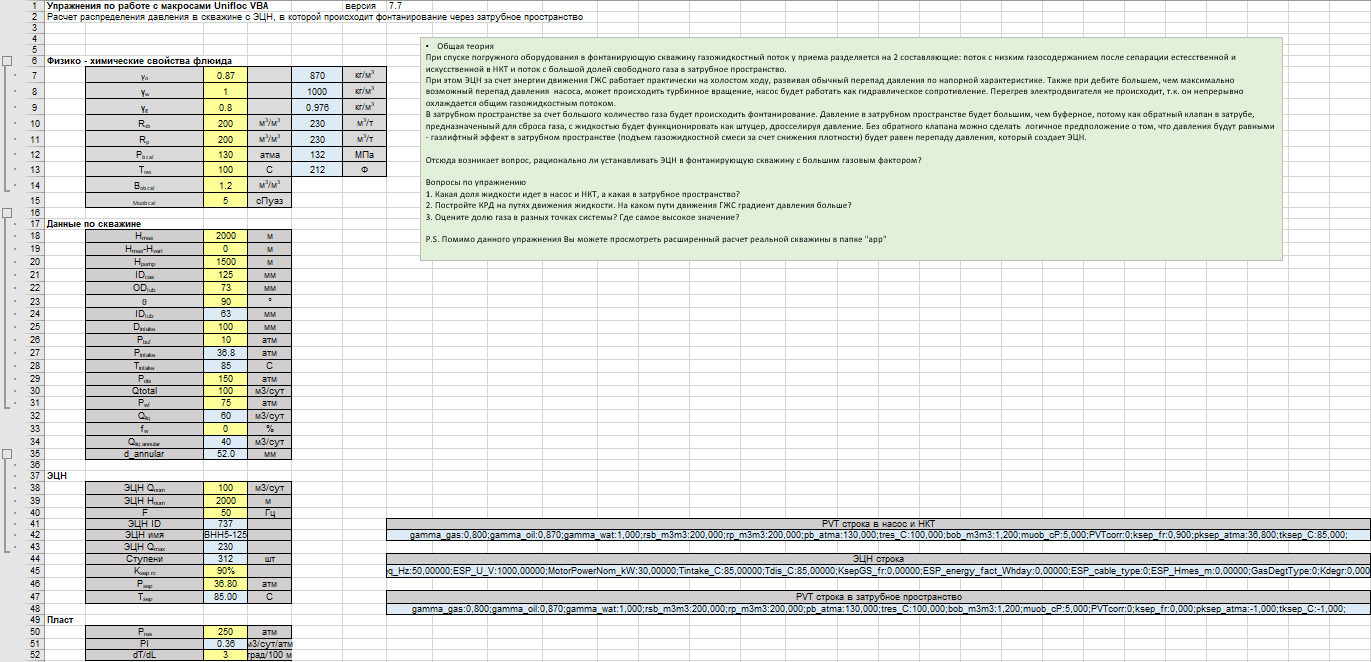
\includegraphics[width=1\linewidth]{Ex110_1}}
	\caption{Набор исходных данных, для расчета фонтанирования через затрубное пространство}
	\label{ris:Ex110_1}
\end{figure}

Процесс моделирования добывающей системы осложняется тем, что неизвестны доли жидкости: поступающая в насос и НКТ и поднимающаяся по затрубному пространству. Для этого введем коэффициент деления потока ГЖС, обозначающий долю жидкости, поступающую в насос и НКТ, в ячейке $N63$. Расчет распределения давления в НКТ и затрубном пространстве будем вести стандартным образом с помощью гидравлических корреляций. Отличия в определении давления будет выражаться в применении двух PVT строк: в ячейке $G42$ будет флюид, учитывающий сепарацию на приеме погружного оборудования, он будет описывать поведение ГЖС в НКТ, а в ячейке $G48$ будет флюид без сепарации - весь газ будет оставаться в потоке в затрубном пространстве; с помощью коэффициента деления потока из общего дебита $Q_{total}$ рассчитывается расход по НКТ $Q_{liq}$ и по затрубному  пространству $Q_{liq annular}$

К формулам, используемым в предыдущем упражнении, добавляется расчет давления в затрубном пространстве (с $Q80$)

{ \small  \texttt{=MF\_p\_pipe\_atma(Q\_annular\_; fw\_; C81;C80; Q81; PVT\_str\_annular\_; theta\_; d\_annular\_pr; 1;D81;D80)
}}

И соответственно доля газа в ГЖС затрубного пространства (с $J81$) 

{ \small  \texttt{=MF\_gas\_fraction\_d(Q81; D81; fw\_; PVT\_str\_annular\_)
}}

Также напомним о важности правильно определения давления сепарации (описано выше). 

Таким образом, с помощью КРД в затрубном пространстве и НКТ предлагается найти такие параметры системы (изменяя коэффициент деления потока, коэффициент деградации напорной характеристики насоса и т.д.) при котором давление в затрубном пространстве будет равным или большим, чем буферное давление.

\begin{figure}[h!]
	\center{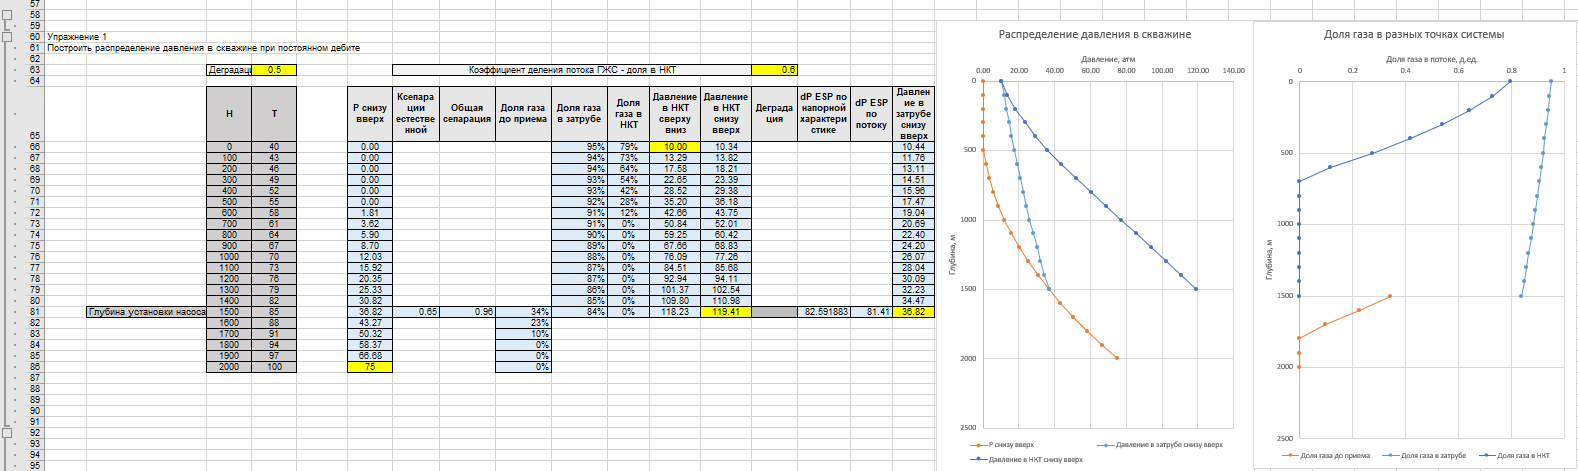
\includegraphics[width=1\linewidth]{Ex110_2}}
	\caption{Настроенная модель скважины с равными давлениями на устье}
	\label{ris:Ex110_2}
\end{figure}

Вопросы по упражнению
\begin{enumerate}
	\item  Какая доля жидкости идет в насос и НКТ, а какая в затрубное пространство?
	\item  Постройте КРД на путях движения жидкости. На каком пути движения ГЖС градиент давления больше?
	\item Оцените долю газа в разных точках системы? Где самое высокое значение?
	\item Оптимальнее ли будет эксплуатировать скважину с помощью чисто фонтанного способа добычи?
\end{enumerate}